%! Author = jannikeschler
%! Date = 18/09/2022

\documentclass[reprint,english,notitlepage]{revtex4-2}
\usepackage{amsmath}
\usepackage[mathletters]{ucs}
\usepackage[utf8x]{inputenc}
\usepackage[english]{babel}
\usepackage{esint}
\usepackage{physics,amssymb}
\usepackage{graphicx}
\usepackage{xcolor}
\usepackage{hyperref}
\usepackage{listings}
\usepackage{subfigure}
\hypersetup{
    colorlinks,
    linkcolor={red!50!black},
    citecolor={blue!50!black},
    urlcolor={blue!80!black}}

\lstset{inputpath=,
	backgroundcolor=\color{white!88!black},
	basicstyle={\ttfamily\scriptsize},
	commentstyle=\color{magenta},
	language=Python,
	morekeywords={True,False},
	tabsize=4,
	stringstyle=\color{green!55!black},
	frame=single,
	keywordstyle=\color{blue},
	showstringspaces=false,
	columns=fullflexible,
	keepspaces=true}

\begin{document}
\title{Simulating Planetary orbits of a solar system}
\author{Jannik Eschler \& Oskar Idland}
\date{\today}
\affiliation{Institute of Theoretical Astrophysics, University of Oslo}

\begin{abstract}
This is an abstract \colorbox{red}{Complete this summary at the end of the paper}
\end{abstract}
\maketitle

\section{Introduction}
When making our way out of the earth's atmosphere, we will have to know where our destination will be after the launch.
To be able to reach our destination we therefore have to get known in our solar system and explore and simulate the different planets in the system.
After finding out the orbits of the planets, it will be much easier to coordinate our launch to our target to minimize the time and effort required to find the destination.
Using this, we will also be able to give estimates about the possibility of extraterrestrial life discovering our solar system.

\section{Method}
The calculation of the planetary orbits in our solar system can either be done numerically or analytically.
Both methods have their advantages and disadvantages compared to the other.
To be able to find the analytical orbit of a planet, we will first have to find an analytical expression for the orbit of a planet.
As planetary orbits usually are ellipses with the star positioned in one of the two foci of the ellipse, we will be able to derive a formula for the position of the planet based on the formula for and ellipse.
An ellipse is defined as "A closed plane curve generated by a point moving in such a way that the sums of its distances from two fixed points is a constant." \colorbox{red}{Merriam Webster}
The analytical expression for an ellipse in cartesian coordinates with the origin in the middle is given by
\begin{align}
    \frac{x^2}{a^2} + \frac{y^2}{b^2} = 1 \label{ellipse_analytic_cart}
\end{align}
For the calculations in this report, it is however advantageous to be able to use this expression in polar coordinates.
When switching to polar coordinates, we will be using the distance $r = |\textbf{r}|$ from the star in one focus point to the point on the ellipse and the angle $f$ at the star from the semi-major axis to the vector $\textbf{r}$ as seen in figure \ref{fig:Ellipse_fig}.
In orbital mechanics, the angle $f$ is also often called the true anomaly.
\begin{figure}[h]
	%% h(here), t(top of page), b(bottom of page)
	\centering
	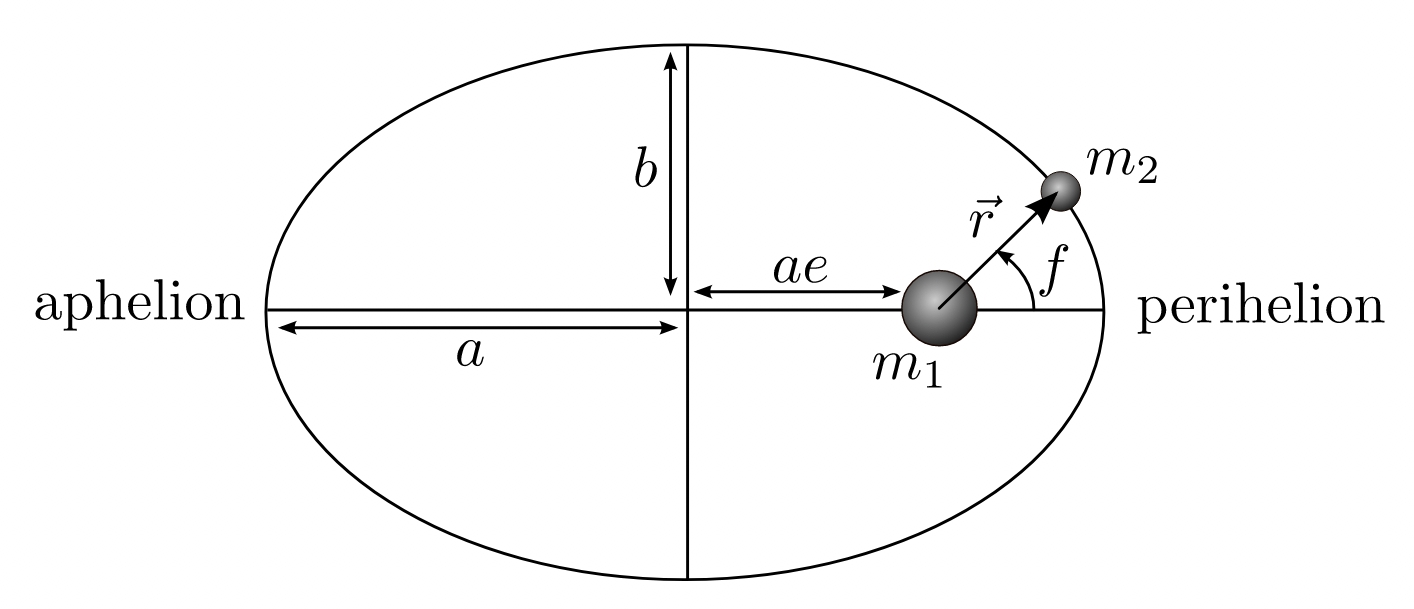
\includegraphics[scale=0.3]{Figures/Ellipse}
	\caption{Figure of an ellipse with all major components}\label{fig:Ellipse_fig}
\end{figure}
Based on figure~\ref{fig:Ellipse_fig} we are now able to see that
\begin{align}
    &x = ae + r\,cos(f) \label{x_ellipse}
\end{align}
\begin{align}
	&y = r\,sin(f) \label{y_ellipse}
\end{align}
Using equations~\ref{x_ellipse} and~\ref{y_ellipse} we wre now able to find an equation for the distance $r$
\begin{align*}
    r = \frac{a(1-e^2)}{1 + e\,cos(f)}
\end{align*}
with e being the eccentricity of the ellipse given by
\begin{align*}
    e = \sqrt{1-\frac{b^2}{a^2}}
\end{align*}
Here, a is the semi-major axis and b is the semi-minor axis of the ellipse.
Now, $r$ can be used to convert the coordinates back to cartesian coordinates using equations~\ref{x_ellipse} and~\ref{y_ellipse}.
By iterating over a collection of equally spaced values between $0$ and $2\pi$, we will find collection of points on the elliptical orbit of the planets, which can then be plotted.
When repeating this for each planet using the given constants for each planet, we will be able to simulate the orbits or all planets.\\\\
The analytical expression, can be used to find the orbit of a given planet, but not the velocity or the position of the planet on the orbit the planet at a given time.
To find the position of the planet in the orbit as a function of time, we will first need to simulate the orbit numerically.
The general idea of the simulation is to use newtons second law $\sum\textbf{F} = m\textbf{a}$ to calculate the acceleration of the planet at a certain position.
In this simulation, all forces except gravitational forces from the star will be neglected.
Therefore the total force exerted on the planet can be calculated using Newtons law of universal gravitation.
\begin{align*}
    &\sum\textbf{F} = G\,\frac{m_1 m_2}{r^2} \label{Newton_Grav_law}\\
	&\sum\textbf{F} = m_1 \textbf{a}\\
	&\bold{a} = G\,\frac{m_1}{r^2}
\end{align*}
With $G$ being the gravitational constant, $m_1$ being the mass of the star, $m_2$ being the mass of the planet, and $r$ being the distance between the star and the planet.\\\\
Using the initial velocity of the object at the position we are calculating the acceleration for, as well as the acceleration, we can find the velocity after a small time interval $\Delta t$.
Correspondingly, using the initial position and velocity, the position after the time step $\Delta t$ can be calculated.
The process is then repeated using the new position and velocity to calculate the acceleration in the point and velocity and position after another time interval $\Delta t$.
There are different variations of this process, with different advantages and disadvantages.\\
In this simulation the Leapfrog method will be used.
This method calculates the acceleration in a point and uses it to find the velocity $\textbf{v}_h$ after $ \frac{dt}{2}$.
Velocity $\textbf{v}_h$ and the initial position of the planet will then be used to calculate the new position after a time interval $\Delta t$.\newline
\begin{figure}[h]
	%% h(here), t(top of page), b(bottom of page)
	\centering
	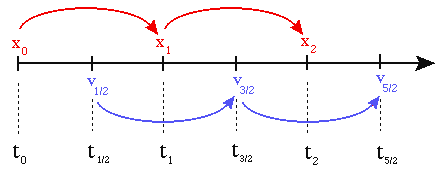
\includegraphics[scale=0.4]{Figures/leapfrog1}
	\caption{\colorbox{red}{Visualisation of the Leapfrog integration algorithm}}\label{fig:Leapfrog_vis}
\end{figure}\newline
As $\textbf{v}_h$ is somewhere between the velocity of the object in the initial position and the position after a time interval $\Delta t$, the calculation of the new position will be more exact.
The process can be described using three equations:
\begin{align*}
    \textbf{a}_i &= A(\textbf{x}_i)\\
	\textbf{v}_{i+1/2} &= \textbf{v}_{i-1/2} + \textbf{a}_i\,\Delta t\\
	\textbf{x}_{i} &= \textbf{x}_i + \textbf{v}_{i+1/2}\,\Delta t
\end{align*}
After simulating the orbits of the planets, the results can be used to find a function of time approximating the orbit of each planet.
This will be done by interpolating the results into a function.\newline \newline

To examine and test the orbits for inaccuracies, we can make use of Johannes Kepler's laws of planetary motion.
The three laws state:
\begin{enumerate}
    \item The orbit of a planet is an ellipse with the
		Sun in one of the foci.
	\item A line connecting the Sun and the planet
		sweeps out equal areas in equal time intervals.
	\item The orbital period around the Sun and the
		semimajor axis of the ellipse are related through:
		\begin{align*}
		    P^2 = a^3
		\end{align*}
		\colorbox{red}{where P is the period in years and a is the
		semimajor axis in Astronomic Units}
\end{enumerate}

First, we will check whether our results agree with Kepler's second law.
To do this, two areas on different sides of the orbit of our home planet,which have been swept out in the same time interval will be compared.\\
To calculate the areas, each area will be divided into smaller areas $dA$, which can be determined by using formula~\eqref{Kepler_dArea}.

\begin{equation} \label{Kepler_dArea}
    dA = \frac{1}{2}r^2 d\theta 
\end{equation}

\colorbox{red}{The derivation of this formula can be found in the Appendix}
When running the simulation, a small area $dA$ which is equal to the area swept out by the position vector $\textbf{r}$ during the time interval $\Delta t$, will be calculated using formula~\eqref{Kepler_dArea}.
To find the total area swept out during a time interval $[a, b]$, all smaller areas $dA$ in the interval $[a, b]$ need to be added together.
This will give an approximation of the total swept out area.
The simulation will calculate the area at two different places in the orbit.
One around the point where the planet is closest to the start, called perihelion, and one around the point the furthest away from the star, called aphelion.\\
The areas should look different, as the planet will have the highest angular velocity at the perihelion and lowest angular velocity at the perihelion.
This is due to the spin of the planet around the star being conserved.
The covered distance and mean velocity of the planet during the interval $[a, b]$, are therefore also interesting measurements, which will be calculated in the simulation.
To do this, the small distances $\Delta \textbf{r}$ which are covered by the planet in the small time intervals $\Delta t$ in the interval $[a, b]$ will therefore be added together.
This will yield in the total distance traveled by the planet in the time interval $[a, b]$.
The mean velocity is found by dividing the total distance by the time $t = b-a$.\newline

Furthermore we will check if the orbits are consistent with Kepler's third law~\eqref{Kepler3} as well as Newtons revised version of Kepler's third law~\eqref{KeplerNewton3}.
Since we have found the rotational period of each planet around the sun using the simulation, we will only have to calculate the rotational period of each planet using Kepler's third law and Newtons revised version and compare them to find out how well they agree.
\begin{align}
    P^2 = a^3 \label{Kepler3}
\end{align}
\begin{align}
	P^2 &= \frac{4 \pi^2}{G \left( m_1 + m_2 \right)} a^3 \label{KeplerNewton3}
\end{align}

To simulate the solar system with the center of mass in origin, we can view this as a N-body system. The simplest example of this is a two-body system where each body has mass $ m_1 , m_2 $ and velocity $ v_1, v_2 $ at position $ r_1, r_2 $. The new system introduces some other new variables. Reduced mass $ \mu $, sum of masses $ M $, the vector $ \mathbf{r} $ from one of the masses, to the other and center of mass $ \mathbf{R} $.
\begin{align*}
	M = m_1 + m_2 \\ \\
	\mathbf{R} = \frac{m_1 \mathbf{r}_1 + m_2  \mathbf{r}_2}{m_1 + m_2} \\ \\
	μ = \frac{m_1 m_2}{M} \\ 
	\mathbf{r} = \mathbf{r}_2 - \mathbf{r}_1
\end{align*}

The kinetic energy $ E_k $ can be written as a sum of the kinetic energy of both bodies.
\[
\mathbf{E_k} = \frac{1}{2}m_1 \mathbf{\dot{r}}_{1}^{2} + \frac{1}{2}m_2 \mathbf{\dot{r}}_{2}^{2}
\]
Using the definition of the center of mass $ \mathbf{R} $ we can redefine the vectors $ \mathbf{r_1} $ and $ \mathbf{r_2} $ to get a new expression for the kinetic energy. For the complete calculations see Appendix \ref{r1r2 calc} and \ref{E_k calc}
\begin{align}
	\mathbf{r}_1 = \mathbf{R} - \frac{m_2}{M}\mathbf{r} \label{r_1 redef} \\
	\mathbf{r}_2 = \mathbf{R} + \frac{m_1}{M}\mathbf{r} \label{r_2 redef}
\end{align}
\[
\mathbf{E_k} = \frac{1}{2}M \mathbf{\dot{R}}^{2} + \frac{1}{2}μ \mathbf{\dot{r}}^{2} 
\]
When putting the center of mass in the origin $ \mathbf{R} = 0 $ and we can simplify further. 
\[
E_k = \frac{1}{2} μ v^{2}
\]

As gravitation is a conservative force the system will have potential energy $ U $. 
\[
U = ∫ _{\infty} ^{r} \frac{Gm_1 m_2}{r^{2}}\mathbf{\hat{r}} ⋅ \mathrm{d}\mathbf{r} = - \frac{GM \mu}{r}
\] 

The total energy can be written as follows. 
\[
E = \frac{1}{2}μ v^{2}  - \frac{GM\mu}{r}
\]

The angular momentum $ \mathbf{P} $ can be expressed as a sum of the angular momentum of the two bodies. 
\[
\mathbf{P} = \mathbf{r}_1 × \mathbf{\dot{r}}_1 + \mathbf{r}_2 × \mathbf{\dot{r}}_2
\]
Using the redefined vectors from \ref{r_1 redef} and \ref{r_2 redef}  we get the following equation. For the full calculation see Appendix \ref{AM calc}
\[
\mathbf{P} = \mathbf{r} × μ \mathbf{\dot{r}}
\]


\section{Results}
\subsection{Planetary Orbits}
    The simulation of the orbits yielded in both numeric and analytic orbits for all planets.
	For both the analytic and the numeric orbits, arrays containing the velocity and position of each planet at \colorbox{red}{N} equally spaced positions along the orbit are returned.
	The simulation then created figure~\ref{fig:Orbit_Plot} from these arrays.
\begin{figure}[h]
	%% h(here), t(top of page), b(bottom of page)
	\centering
	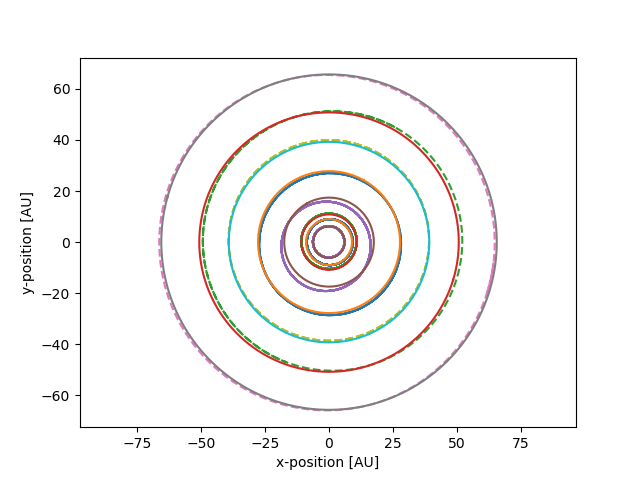
\includegraphics[scale=0.4]{Figures/Orbit_plots}
	\caption{Plot of the simulated orbits of our solar system}\label{fig:Orbit_Plot}
\end{figure}\\
	The star is denoted by the black dot in the middle of the solar system.
	Around the star, there are 8 sets of orbits, one set for each planet.
	The numeric orbit for each planet is represented by a dashed line, whereas the analytic orbis is represented by a solid line.\\
	The numeric and analytic orbits are slightly elliptic, and line up quite well for all planets, with only some deviance.
	As seen in Figure~\ref{fig:Orbit_Plot}, they have the same shapes, but appear not to be entirely concentric.

\subsection{Comparison to Kepler's Laws}
	To compare the orbit of our home planet to Kepler's second law, two different areas $A$ swept out by the position vector $ \textbf{r}$ during the same time interval have been calculated.
	Furthermore, the covered distance and mean velocity during each time interval have been calculated and are shown in table~\ref{tab:Kepler2_table1}.
	The differences between the values of each area are presented in table~\ref{tab:Kepler2_table2}. Areas are given in AU$^2$, Distances in AU and Velocities in AU/Yr.
\begin{table}[h]
	%% l (Left aligned), c (Centered), r (Right aligned)
    \begin{tabular}{ |c|c|c| }
		\hline
        Planet 0 & Aphelion & Perihelion\\
        \hline
        Area & 0.00000307 & 0.00000307\\
        \hline
		Distance & 6.823815E-07 & 6.823823E-07\\
		\hline
		Velocity & 0.20996355 & 0.20996378\\
		\hline
    \end{tabular}
	\caption{Area, Distance and Velocity results for calculated areas at Aphelion and Perihelion}
	\label{tab:Kepler2_table1}
\end{table}

\begin{table}[h]
    \begin{tabular}{ |c|c| }
		\hline
		 & Difference\\
		\hline
		Area & 3.181500E-12 AU^2\\
		\hline
		Distance & 7.306208E-13 AU\\
		\hline
		Velocity & 0.00000022 AU/Yr\\
		\hline
	\end{tabular}
    \caption{Differences between results of the two areas}
    \label{tab:Kepler2_table2}
\end{table}\\

	To check whether the calculated orbits agree with Kepler's third law and Newton's revised version of Kepler's third law, the orbital period has been calculated analytically and using each of the two laws~\eqref{Kepler3} and~\eqref{KeplerNewton3} for each planet.
	This yields in the following results.\\

\begin{table}[h]
    \begin{tabular}{ |c|c|c| }
        %% l (Left aligned), c (Centered), r (Right aligned)
        \hline
		Method & \textbf{Planet 0} & \textbf{Planet 1}\\
		\hline
        Analytic	& 12.81499 Yrs & 16.93432 Yrs\\
		Kepler		& 27.00534 Yrs & 35.68609 Yrs\\
		Newton		& 12.81498 Yrs & 16.93431 Yrs\\
		\hline\hline
		Method & \textbf{Planet 2} & \textbf{Planet 3}\\
		\hline
        Analytic	& 34.83863 Yrs & 252.32753 Yrs\\
		Kepler		& 73.41629 Yrs & 531.73585 Yrs\\
		Newton		& 34.83862 Yrs & 252.32499 Yrs\\
		\hline\hline
		Method & \textbf{Planet 4} & \textbf{Planet 5}\\
		\hline
        Analytic	& 116.61089 Yrs & 69.47113 Yrs\\
		Kepler		& 245.73693 Yrs & 146.39819 Yrs\\
		Newton		& 116.61089 Yrs & 69.47113 Yrs\\
		\hline\hline
		Method & \textbf{Planet 6} & \textbf{Planet 7}\\
		\hline
        Analytic	& 171.66819 Yrs & 7.25601 Yrs\\
		Kepler		& 361.76050 Yrs & 15.29077 Yrs\\
		Newton		& 171.66798 Yrs & 7.25601 Yrs\\
		\hline
	\end{tabular}
    \caption{Orbital Periods of all planets calculated using three different methods}
    \label{tab:Kepler3_Table}
\end{table}


\\It can be seen that the orbits are not entirely consistent with Kepler's third law.
They are however very consistent with Newton's revised version of Kepler's third law as they deviate less than $0.0015\%$ from each other.



\section{Discussion}
To get an accurate simulation, it is important to choose a sufficiently small time interval dt.
An adequate number is approximately 10'000 steps per year of simulation, which corresponds to a time interval of $\Delta t = 52$ min $33.6$ sec.
Using smaller time intervals will result in a more precise simulation, but will increase computing time. In this simulation, $3*10^6$ time steps were used over a time period of $260$ Years.
This will result in a time step of $\Delta t = 45$ min $35$ sec, which seems reasonable.
The simulation has then been run once with $8*10^7$ time steps, which did not result in any significant change in the results but reduced the time interval to $\Delta t = 1$ min $46$ sec.
Due to the large dimensions of the orbits, this is enough to be able to simulate the orbits precisely.\\
These orbits will, however, not be entirely as it would be in reality, due to the fact that we are using some simplifications.
The most important being negation of relativistic effects and assuming that there are no forces other than the gravitational force from the sun.
In reality, there would be interplanetary forces, which would affect the orbit of each planet.
Solar winds might also affect the movement of the planets, especially those who are close to the star.\\
When comparing the results from the simulation to the results calculated using Kepler's second and third law as well as Newtons revised version of it, we see some deviance.
The Distances covered and velocities of our home planet while sweeping out the two areas are as expected quite different.
However, the areas only differentiate by approximately $0.0001\%$.\\

The analytically calculated orbital time of the planets differ quite a lot from the time calculated using Kepler's third law.
The relative difference is approximately $110.733 \pm 0.001\%$ for all planets.
So the relative difference is almost the same for all planets.
Newton's revised version, gives a better result and results in the relative difference being approximately $0.0005 \pm 0.001\%$ for all planets, which is very accurate.
This makes sense since we are not working with earth, but rather another home planet, which requires a more general formula.

	\subsection{Subsection}

\section{Conclusion}
And the conclusion

\section{References}
References are important!
\begin{enumerate}
	\item \url{https://www.merriam-webster.com/dictionary/ellipse}
	\item \url{https://cvarin.github.io/CSci-Survival-Guide/leapfrog.html}
	\item \url{https://www.uio.no/studier/emner/matnat/astro/AST2000/h22/undervisningsmateriell/lecture_notes/part1b.pdf}
\end{enumerate}

\section{Appendix: Mathematical Derivations}
	\subsection{Calculations}
		\subsubsection{Redefining $ \mathbf{r_1} $ and $ \mathbf{r_2} $}\label{r1r2 calc}
			\[
			\mathbf{R} = \frac{m_1 \mathbf{r_1} + m_2 \mathbf{r_2}}{M}, \qquad \mathbf{r} = \mathbf{r_2} - \mathbf{r_1}
			\]
			\[
			\mathbf{R} = \frac{m_1}{M}\mathbf{r_1} + \frac{m_2}{M} \left( \mathbf{r} + \mathbf{r_1} \right) = \mathbf{r_1} \left( \frac{m_1 + m_2}{M} \right) + \frac{m_2}{M} \mathbf{r} = \mathbf{r_1} + \frac{m_2}{M} \mathbf{r}
			\]
			\[
			r_1 = \mathbf{R} - \frac{m_2}{M}\mathbf{r}
			\]
			Repeating the same calculations for $ r_2 $ yields the following: 
			\[
			r_2 = \mathbf{R} + \frac{m_1}{M} \mathbf{r}
			\]

		\subsubsection{Calculating Kinetic Energy}\label{E_k calc}
			\[
				\mathbf{E_k} = \frac{1}{2}m_1 \mathbf{\dot{r}}_{1}^{2} + \frac{1}{2}m_2 \mathbf{\dot{r}}_{2}^{2}
			\]
			Substituting the new definitions of $ \mathbf{r}_1 $ and $ \mathbf{r}_2 $ from \ref{r_1 redef} and  \ref{r_2 redef}.
			\[
			\mathbf{E_k} = \frac{1}{2} m_1 \left(\mathbf{\dot{R}} - \frac{m_2}{M}\mathbf{\dot{r}}\right)_{}^{2} + \frac{1}{2} m_2 \left(\mathbf{\dot{R}} + \frac{m_1}{M} \mathbf{\dot{r}}\right)_{}^{2}
			\]
			\[
			\mathbf{E_k} = \frac{1}{2} \left(m_1 \mathbf{\dot{R}}^{2} - \frac{2m_1 m_2}{M}\mathbf{\dot{r}}^{2} + \frac{m_1m_2^{2}}{M^{2}}\mathbf{\dot{r}}^{2} + \frac{2m_1m_2}{M}\mathbf{\dot{r}}^{2} + \frac{m_2m_1^{2}}{M^{2}}\right)_{}^{}
			\]
			\[
			\mathbf{E_k} = \frac{1}{2}\left( m_1 + m_2 \right) \mathbf{\dot{R}} + \frac{1}{2} \frac{m_1m_2}{M^{2}} \left( m_1+ m_2  \right) \mathbf{\dot{r}}^{2}
			\]
			\[
			\mathbf{E_k} = \frac{1}{2} M \mathbf{\dot{R}}^{2} + \frac{1}{2} μ \mathbf{\dot{r}}^{2}
			\]
			When the center of mass is put in the origin $ \mathbf{R} = 0 $.
			\[
			E_k = \frac{1}{2} μ v^{2}
			\]


		\subsubsection{Calculating Angular Momentum}\label{AM calc}
			\[
			\mathbf{P} = m_1 \left(- \frac{m_2}{M}\right)_{}^{2}\mathbf{r_1} × \mathbf{\dot{r}} + m_2 \left(\frac{m_1}{M}\right)_{}^{2} \mathbf{r_2} × \mathbf{\dot{r}}
			\]
			\[
			\mathbf{P} = \frac{m_1m_2}{M^{2}} \left(m_1 + m_2\right)_{}^{} \mathbf{r} × \mathbf{\dot{r}} 
			\]
			\[
			\mathbf{P} = μ \mathbf{r} = \mathbf{\dot{r}}
			\]
			\[
			\mathbf{P} = \mathbf{r} × μ \mathbf{\dot{r}}
			\]


\end{document}